\documentclass[tikz,convert={density=300,outfile=\jobname.png}]{standalone}
\usepackage[utf8]{inputenc}		% bei der Verw. von lualatex oder xelatex entfernen!
\usepackage{tikz}

\usetikzlibrary{calc}

\usetikzlibrary{shapes.geometric}
\usetikzlibrary{positioning}

\begin{document}
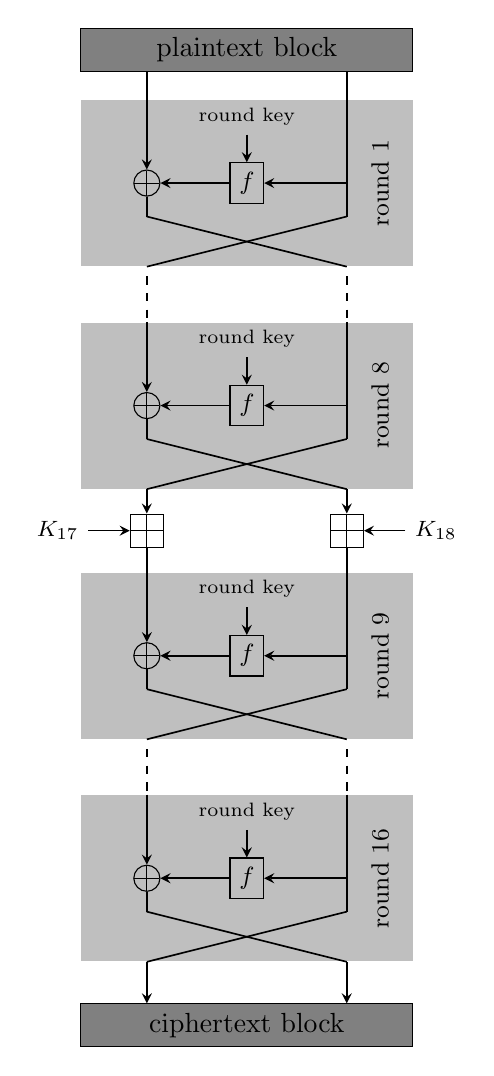
\begin{tikzpicture}

\tikzset{
    myarrow/.style={-{stealth}, semithick},
    myarrowdashed/.style={semithick, dashed},
    myline/.style={semithick},
    triangle/.style = {draw, regular polygon, regular polygon sides=3, inner sep=0pt, minimum height=130},
    node rotated/.style = {rotate=180},
    border rotated/.style = {shape border rotate=180},
     pre/.style={<-,shorten <=1pt,>=stealth',semithick},
     post/.style={->,shorten >=1pt,>=stealth',semithick}
}

\tikzset{XOR/.style={draw,circle,append after command={
        [shorten >=\pgflinewidth, shorten <=\pgflinewidth, semithick,]
        (\tikzlastnode.north) edge (\tikzlastnode.south)
        (\tikzlastnode.east) edge (\tikzlastnode.west)
        }
    }
}

\tikzset{BOXPLUS/.style={draw,rectangle, inner sep=6pt,append after command={
        [shorten >=\pgflinewidth, shorten <=\pgflinewidth, semithick,]
        (\tikzlastnode.north) edge (\tikzlastnode.south)
        (\tikzlastnode.east) edge (\tikzlastnode.west)
        }
    }
} 


\pgfmathsetmacro{\D}{10}
\pgfmathsetmacro{\W}{120}
\pgfmathsetmacro{\H}{60}
\pgfmathsetmacro{\A}{50}
 
%******************** 
   % Beginning of drawing
%********************

%ANCHOR TOP
\node [draw, fill=gray, minimum width=\W pt] (kBlock) {plaintext block};

%BEGIN ROUND 1 BOX
\node [fill=lightgray, below=\D pt of kBlock.south, anchor=north, minimum width=\W pt, minimum height=\H pt](round1Block) {};

%ANCHOR TOP LEFT
\path let \p0 = ($ (kBlock.south west)!0.20!(kBlock.south east) $)
	in node [] (kanch1) at (\p0) {};

%ANCHOR TOP RIGHT	
\path let \p0 = ($ (kBlock.south west)!0.80!(kBlock.south east) $)
	in node [] (kanch2) at (\p0) {};

% F1
\path let \p0 = ($ (round1Block.south)!0.50!(round1Block.north) $)
	in node [draw] (f1) at (\p0) {\small $f$};
% XOR ROUND 1
\path let
	\p0 = (kanch1),
	\p1 = (f1)
	in node [XOR] (r1fconleft) at (\x0 ,\y1) {};
	
	
%ROUND KEY
\path let
	\p0 = (f1),
	\p1 = ($ (round1Block.south)!0.90!(round1Block.north) $)
	in node [] (roundK1) at (\x0 ,\y1) {\scriptsize round key};

%Point before twist LEFT
\path let
	\p0 = (r1fconleft),
	\p1 = ($ (round1Block.south)!0.30!(round1Block.north) $)
	in node [] (r1conleft) at (\x0 ,\y1) {};

% BRANCH ABOVE RIGHT LINE
\path let
	\p0 = (kanch2),
	\p1 = (f1)
	in node [] (r1fconright) at (\x0 ,\y1) {};	
	
% DESCRIPTION
\path let
	\p0 = ($ (r1fconright.center)!0.50!(round1Block.east) $),
	\p1 = (f1)
	in node [rotate=90] (descr) at (\x0 ,\y1) {\small round 1};

%Point before twist LEFT
\path let
	\p0 = (kanch2),
	\p1 = ($ (round1Block.south)!0.30!(round1Block.north) $)
	in node [] (r1conright) at (\x0 ,\y1) {};
	
%TWISTER
\path let
	\p0 = (r1fconleft),
	\p1 = (round1Block.south)
	in node [] (r1twistleft) at (\x0 ,\y1) {};
	
\path let
	\p0 = (r1fconright),
	\p1 = (round1Block.south)
	in node [] (r1twistright) at (\x0 ,\y1) {};
	
%%% DRAW LINES ROUND 1
\draw[myarrow] (kanch1.center) -- (r1fconleft.north);
\draw[myline] (kanch2.center) -- (r1fconright.center);
\draw[myarrow] (r1fconright.center) -- (f1.east);
\draw[myarrow] (f1.west) -- (r1fconleft.east);
\draw[myline] (r1fconleft.south) -- (r1conleft.center);
\draw[myline] (r1fconright.center) -- (r1conright.center);
\draw[myline] (r1conleft.center) -- (r1twistright.center);
\draw[myline] (r1conright.center) -- (r1twistleft.center);
\draw[myarrow] (roundK1) -- (f1.north);


%%%%%%%%%%%%%%%%%%%%%%%%%%%%%%%%%%%%%%%%%%%%%
%BEGIN ROUND 2 BOX
%%%%%%%%%%%%%%%%%%%%%%%%%%%%%%%%%%%%%%%%%%%%%
\node [fill=lightgray, below=\D * 2 pt of round1Block.south, anchor=north, minimum width=\W pt, minimum height=\H pt](round2Block) {};

%ANCHOR TOP LEFT
\path let \p0 = ($ (round2Block.north west)!0.20!(round2Block.north east) $)
	in node [] (r2kanch1) at (\p0) {};

%ANCHOR TOP RIGHT	
\path let \p0 = ($ (round2Block.north west)!0.80!(round2Block.north east) $)
	in node [] (r2kanch2) at (\p0) {};


% F2
\path let \p0 = ($ (round2Block.south)!0.50!(round2Block.north) $)
	in node [draw] (f2) at (\p0) {\small $f$};
% XOR ROUND 1
\path let
	\p0 = (kanch1),
	\p1 = (f2)
	in node [XOR] (r2fconleft) at (\x0 ,\y1) {};
	
%ROUND KEY
\path let
	\p0 = (f2),
	\p1 = ($ (round2Block.south)!0.90!(round2Block.north) $)
	in node [] (roundK2) at (\x0 ,\y1) {\scriptsize round key};

% DESCRIPTION
\path let
	\p0 = ($ (r1fconright.center)!0.50!(round1Block.east) $),
	\p1 = (f2)
	in node [rotate=90] (descr) at (\x0 ,\y1) {\small round 8};

%Point before twist LEFT
\path let
	\p0 = (r2fconleft),
	\p1 = ($ (round2Block.south)!0.30!(round2Block.north) $)
	in node [] (r2conleft) at (\x0 ,\y1) {};

% BRANCH ABOVE RIGHT LINE
\path let
	\p0 = (kanch2),
	\p1 = (f2)
	in node [] (r2fconright) at (\x0 ,\y1) {};	

%Point before twist LEFT
\path let
	\p0 = (kanch2),
	\p1 = ($ (round2Block.south)!0.30!(round2Block.north) $)
	in node [] (r2conright) at (\x0 ,\y1) {};
	
%TWISTER
\path let
	\p0 = (r2fconleft),
	\p1 = (round2Block.south)
	in node [] (r2twistleft) at (\x0 ,\y1) {};
	
\path let
	\p0 = (r1fconright),
	\p1 = (round2Block.south)
	in node [] (r2twistright) at (\x0 ,\y1) {};
	
	
%DASHED%
\draw[myarrowdashed] (r1twistleft) -- (r2kanch1.center);
\draw[myarrowdashed] (r1twistright) -- (r2kanch2.center);

%%% DRAW LINES ROUND 2
\draw[myarrow] (r2kanch1.center) -- (r2fconleft.north);
\draw[myline] (r2kanch2.center) -- (r2fconright.center);
\draw[myarrow] (r2fconright.center) -- (f2.east);
\draw[myarrow] (f2.west) -- (r2fconleft.east);
\draw[myline] (r2fconleft.south) -- (r2conleft.center);
\draw[myline] (r2fconright.center) -- (r2conright.center);
\draw[myline] (r2conleft.center) -- (r2twistright.center);
\draw[myline] (r2conright.center) -- (r2twistleft.center);
\draw[myarrow] (roundK2) -- (f2.north);


%%%%%%%%%%%%%%%%%%%%%%%%%%%%%%%%%%%%%%%%%%%%%
%BEGIN ROUND 3 BOX
%%%%%%%%%%%%%%%%%%%%%%%%%%%%%%%%%%%%%%%%%%%%%
\node [fill=lightgray, below=\D * 3 pt of round2Block.south, anchor=north, minimum width=\W pt, minimum height=\H pt](round3Block) {};

%ANCHOR TOP LEFT
\path let \p0 = ($ (round3Block.north west)!0.20!(round3Block.north east) $)
	in node [] (r3kanch1) at (\p0) {};

%ANCHOR TOP RIGHT	
\path let \p0 = ($ (round3Block.north west)!0.80!(round3Block.north east) $)
	in node [] (r3kanch2) at (\p0) {};


% F2
\path let \p0 = ($ (round3Block.south)!0.50!(round3Block.north) $)
	in node [draw] (f3) at (\p0) {\small $f$};
% XOR ROUND 1
\path let
	\p0 = (kanch1),
	\p1 = (f3)
	in node [XOR] (r3fconleft) at (\x0 ,\y1) {};
	
%ROUND KEY
\path let
	\p0 = (f3),
	\p1 = ($ (round3Block.south)!0.90!(round3Block.north) $)
	in node [] (roundK3) at (\x0 ,\y1) {\scriptsize round key};

% DESCRIPTION
\path let
	\p0 = ($ (r1fconright.center)!0.50!(round1Block.east) $),
	\p1 = (f3)
	in node [rotate=90] (descr) at (\x0 ,\y1) {\small round 9};

%Point before twist LEFT
\path let
	\p0 = (r3fconleft),
	\p1 = ($ (round3Block.south)!0.30!(round3Block.north) $)
	in node [] (r3conleft) at (\x0 ,\y1) {};

% BRANCH ABOVE RIGHT LINE
\path let
	\p0 = (kanch2),
	\p1 = (f3)
	in node [] (r3fconright) at (\x0 ,\y1) {};	

\path let
	\p0 = (kanch2),
	\p1 = ($ (round3Block.south)!0.30!(round3Block.north) $)
	in node [] (r3conright) at (\x0 ,\y1) {};
	
%TWISTER
\path let
	\p0 = (r3fconleft),
	\p1 = (round3Block.south)
	in node [] (r3twistleft) at (\x0 ,\y1) {};
	
\path let
	\p0 = (r3fconright),
	\p1 = (round3Block.south)
	in node [] (r3twistright) at (\x0 ,\y1) {};
	

%%% DRAW LINES ROUND 2
\draw[myarrow] (r3kanch1.center) -- (r3fconleft.north);
\draw[myline] (r3kanch2.center) -- (r3fconright.center);
\draw[myarrow] (r3fconright.center) -- (f3.east);
\draw[myarrow] (f3.west) -- (r3fconleft.east);
\draw[myline] (r3fconleft.south) -- (r3conleft.center);
\draw[myline] (r3fconright.center) -- (r3conright.center);
\draw[myline] (r3conleft.center) -- (r3twistright.center);
\draw[myline] (r3conright.center) -- (r3twistleft.center);
\draw[myarrow] (roundK3) -- (f3.north);



%%%%%%%%%%%%%%%%%%%%%%%%%%%%%%%%%%%%%%%%%%%%%%
%%%%%%%%%%%% BOXPLUS CONNECTORS %%%%%%%%%%%%%%
%%%%%%%%%%%%%%%%%%%%%%%%%%%%%%%%%%%%%%%%%%%%%%

%BOXPLUS LEFT
\path let
	\p0 = (kanch1),
	\p1 = ($ (round2Block.south)!0.50!(round3Block.north) $)
	in node [BOXPLUS] (boxplus1) at (\x0 ,\y1) {};

\path let
	\p0 = (kanch2),
	\p1 = ($ (round2Block.south)!0.50!(round3Block.north) $)
	in node [BOXPLUS] (boxplus2) at (\x0 ,\y1) {};
	
\node[left=15pt of boxplus1, anchor=east, align=center] (keyboxplus1) {\footnotesize $K_{17}$};
\node[right=15pt of boxplus2, anchor=west, align=center] (keyboxplus2) {\footnotesize $K_{18}$};		

	
\draw[myarrow] (r2twistleft.center) -- (boxplus1.north);
\draw[myarrow] (r2twistright.center) -- (boxplus2.north);
\draw[myline] (boxplus1.south) -- (r3kanch1.center);
\draw[myline] (boxplus2.south) -- (r3kanch2.center);

\draw[myarrow] (keyboxplus1) edge (boxplus1);
\draw[myarrow] (keyboxplus2) edge (boxplus2);


%%%%%%%%%%%%%%%%%%%%%%%%%%%%%%%%%%%%%%%%%%%%%
%BEGIN ROUND 4 BOX
%%%%%%%%%%%%%%%%%%%%%%%%%%%%%%%%%%%%%%%%%%%%%
\node [fill=lightgray, below=\D * 2 pt of round3Block.south, anchor=north, minimum width=\W pt, minimum height=\H pt](round4Block) {};

%ANCHOR TOP LEFT
\path let \p0 = ($ (round4Block.north west)!0.20!(round4Block.north east) $)
	in node [] (r4kanch1) at (\p0) {};

%ANCHOR TOP RIGHT	
\path let \p0 = ($ (round4Block.north west)!0.80!(round4Block.north east) $)
	in node [] (r4kanch2) at (\p0) {};


% F2
\path let \p0 = ($ (round4Block.south)!0.50!(round4Block.north) $)
	in node [draw] (f4) at (\p0) {\small $f$};
% XOR ROUND 1
\path let
	\p0 = (kanch1),
	\p1 = (f4)
	in node [XOR] (r4fconleft) at (\x0 ,\y1) {};
	
%ROUND KEY
\path let
	\p0 = (f4),
	\p1 = ($ (round4Block.south)!0.90!(round4Block.north) $)
	in node [] (roundK4) at (\x0 ,\y1) {\scriptsize round key};
	

% DESCRIPTION
\path let
	\p0 = ($ (r1fconright.center)!0.50!(round1Block.east) $),
	\p1 = (f4)
	in node [rotate=90] (descr) at (\x0 ,\y1) {\small round 16};

%Point before twist LEFT
\path let
	\p0 = (r4fconleft),
	\p1 = ($ (round4Block.south)!0.30!(round4Block.north) $)
	in node [] (r4conleft) at (\x0 ,\y1) {};

% BRANCH ABOVE RIGHT LINE
\path let
	\p0 = (kanch2),
	\p1 = (f4)
	in node [] (r4fconright) at (\x0 ,\y1) {};	

\path let
	\p0 = (kanch2),
	\p1 = ($ (round4Block.south)!0.30!(round4Block.north) $)
	in node [] (r4conright) at (\x0 ,\y1) {};
	
%TWISTER
\path let
	\p0 = (r4fconleft),
	\p1 = (round4Block.south)
	in node [] (r4twistleft) at (\x0 ,\y1) {};
	
\path let
	\p0 = (r4fconright),
	\p1 = (round4Block.south)
	in node [] (r4twistright) at (\x0 ,\y1) {};
	
	
%DASHED%
\draw[myarrowdashed] (r3twistleft) -- (r4kanch1.center);
\draw[myarrowdashed] (r3twistright) -- (r4kanch2.center);

%%% DRAW LINES ROUND 2
\draw[myarrow] (r4kanch1.center) -- (r4fconleft.north);
\draw[myline] (r4kanch2.center) -- (r4fconright.center);
\draw[myarrow] (r4fconright.center) -- (f4.east);
\draw[myarrow] (f4.west) -- (r4fconleft.east);
\draw[myline] (r4fconleft.south) -- (r4conleft.center);
\draw[myline] (r4fconright.center) -- (r4conright.center);
\draw[myline] (r4conleft.center) -- (r4twistright.center);
\draw[myline] (r4conright.center) -- (r4twistleft.center);
\draw[myarrow] (roundK4) -- (f4.north);


%ANCHOR BOTTOM
\node [draw, fill=gray, minimum width=\W pt, below=\D *1.5 pt of round4Block.south, anchor=north] (cBlock) {ciphertext block};

\path let \p0 = ($ (cBlock.north west)!0.20!(cBlock.north east) $)
	in node [] (r5kanch1) at (\p0) {};

%ANCHOR TOP RIGHT	
\path let \p0 = ($ (cBlock.north west)!0.80!(cBlock.north east) $)
	in node [] (r5kanch2) at (\p0) {};
	
\draw[myarrow] (r4twistleft.center) -- (r5kanch1.center);
\draw[myarrow] (r4twistright.center) -- (r5kanch2.center);

\end{tikzpicture}
\end{document}